%%%%%%%%%%%%%%%%%%%%%%%%%%%%%%%%%%%%%%%%%%%%%%%%%%%%%%%%%%%%%%%%%%%%%%%%%%%

\chapter{Number Theory}


%%%%%%%%%%%%%%%%%%%%%%%%%%%%%%%%%%%%%%%%%%%%%%%%%%%%%%%%%%%%%%%%%%%%%%%%%%%

\section{Integers}

An \emph{integer} is a whole number. It can be positive, negative, or
zero. Examples of integers include $-13$, $-1$, $0$, and $42$. When we
talk about all the whole numbers, we can use the name \emph{integer}
to refer to them, or we can list all the whole numbers like so:
\[
\dots, -4, -3, -2, -1, 0, 1, 2, 3, 4, \dots
\]
But for convenience, we usually write $\ZZ$ to denote the set of all
integers:
\[
\ZZ
=
\{\dots, -3, -2, -1, 0, 1, 2, 3, \dots\}.
\]
In Sage, the set of all integers is represented as \verb!ZZ! and a
single integer is represented using \verb!Integer!:
%
\begin{lstlisting}
sage: ZZ
Integer Ring
sage: type(ZZ)
<type 'sage.rings.integer_ring.IntegerRing_class'>
sage: 1 in ZZ
True
sage: -1 in ZZ
True
sage: 3.1415 in ZZ
False
sage: type(3)
<type 'sage.rings.integer.Integer'>
sage: Integer
<type 'sage.rings.integer.Integer'>
\end{lstlisting}
%
Notice that in the above code listing, we used \verb!in! to test
whether or not a number is an integer. The command
%
\begin{lstlisting}
sage: 1 in ZZ
True
\end{lstlisting}
%
gives the result \verb!True! because $1$ is an integer. On the other
hand, the command
%
\begin{lstlisting}
sage: 3.1415 in ZZ
False
\end{lstlisting}
%
gives \verb!False! because $3.1415$ is not an integer.


%%%%%%%%%%%%%%%%%%%%%%%%%%%%%%%%%%%%%%%%%%%%%%%%%%%%%%%%%%%%%%%%%%%%%%%%%%%

\section{Prime numbers}

A positive integer $n > 1$ is a \emph{prime} number if its factors are
exclusively $1$ and itself. The integer $2$ is prime because its only
factors are $1$ and $2$. As a matter of fact, $2$ is the smallest
prime integer. The next prime after $2$ is $3$. However, the next
integer $4$ is not prime because $2$ is a factor of $4$. In Sage, the
command \verb!is_prime! tests whether or not an integer is prime. We
can obtain the first $15$ prime numbers using the command
\verb!primes_first_n!.

\begin{lstlisting}
sage: is_prime(1)
False
sage: is_prime(2)
True
sage: is_prime(3)
True
sage: is_prime(4)
False
sage: primes_first_n(15)
[2, 3, 5, 7, 11, 13, 17, 19, 23, 29, 31, 37, 41, 43, 47]
\end{lstlisting}

If $n$ is an integer, the command \verb!next_prime! can be used to
compute the next prime integer starting from $n$. Likewise, the command
\verb!previous_prime! computes the previous prime integer starting
from $n$.
%
\begin{lstlisting}
sage: next_prime(-25)
2
sage: next_prime(1)
2
sage: next_prime(50)
53
sage: previous_prime(50)
47
sage: previous_prime(3)
2
sage: previous_prime(2)
Traceback (most recent call last):
...
ValueError: no previous prime
\end{lstlisting}
%
The command
%
\begin{lstlisting}
sage: next_prime(-25)
2
\end{lstlisting}
%
results in \verb!2! because $2$ is the smallest prime. In other words,
there are no primes smaller than $2$, which explains the result of the
following command:
%
\begin{lstlisting}
sage: previous_prime(2)
Traceback (most recent call last):
...
ValueError: no previous prime
\end{lstlisting}

There are various questions we can ask about prime numbers. For
example, how many prime integers are there? Over two thousand years
ago, the Greek mathematician Euclid proved that there are infinitely
many primes. No matter how high up we count, there is still a prime
number to be found.

Here's another question: If $n$ is a positive integer greater than
$1$, how many primes are there between $1$ and $n$? In the case of $n
= 50$, we could use the command \verb!primes_first_n! to list the
first 20 primes, then count how many of those primes are less than or
equal to $50$.
%
\begin{lstlisting}
sage: primes_first_n(20)
[2, 3, 5, 7, 11, 13, 17, 19, 23, 29, 31, 37, 41, 43, 47, 53, 59, 61, 67, 71]
sage: P = [2, 3, 5, 7, 11, 13, 17, 19, 23, 29, 31, 37, 41, 43, 47]; P
[2, 3, 5, 7, 11, 13, 17, 19, 23, 29, 31, 37, 41, 43, 47]
sage: len(P)
15
\end{lstlisting}
%
In the above code listing, we put all the primes less than or equal to
$50$ into the list \verb!P!. We then used the command \verb!len! to
obtain the length of that list. From the above output, there are $15$
primes less than or equal to $n = 50$.

Alternatively, we can let the command \verb!prime_pi! do all the hard
work for us. Given an integer $n$---either positive, negative, or
zero---the command \verb!prime_pi(n)! counts how many primes are less
than or equal to $n$.
%
\begin{lstlisting}
sage: prime_pi(50)
15
sage: prime_pi(100)
25
sage: prime_pi(1000)
168
sage: prime_pi(10000)
1229
sage: prime_pi(0)
0
sage: prime_pi(-10)
0
\end{lstlisting}
%
To study the output of \verb!prime_pi(n)! as the integer \verb!n!
increases, we could substitute $n = 1, 2, 3, \dots$ into the
command. Or we could use \verb!plot! together with \verb!prime_pi! to
visualize how the output of \verb!prime_pi! changes as $n$ increases
in value. Figure~\ref{fig:number_theory:prime_pi_for_n_leq_100}
illustrates the change in the values of \verb!prime_pi! as $n$ takes
on all integer values from $0$ up to and including $100$. Notice that
when $n = 50$, the output of \verb!prime_pi! is $15$, which confirms
our computation above. The horizontal axis shows integer values of $n$
from $0$ to $100$, inclusive, while the vertical axis shows the output
of the command \verb!prime_pi(n)!. The figure was produced using the
following code listing:
%
\begin{lstlisting}
sage: P = plot(prime_pi, 0, 100)
sage: V = line([(50,0), (50,25)], color="red")     # vertical line
sage: H = plot(15, xmin=0, xmax=100, color="red")  # horizontal line
sage: P + H + V
\end{lstlisting}
%
\begin{figure}[!htbp]
\centering
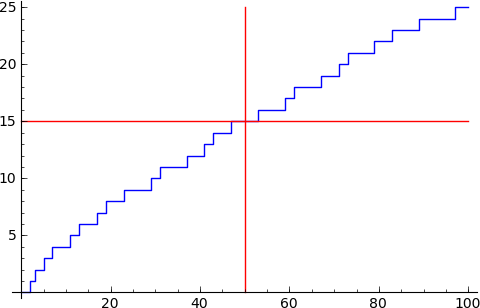
\includegraphics[scale=0.8]{images/prime-pi-100}
\caption{Values of \texttt{prime\_pi(n)} for $n = 0, 1, 2, \dots, 100$.}
\label{fig:number_theory:prime_pi_for_n_leq_100}
\end{figure}
%
And Figure~\ref{fig:number_theory:prime_pi_for_n_leq_1000} shows the
behavior of \verb!prime_pi! as $n$ increases from $0$ to $1000$. The
figure was produced using the command:
%
\begin{lstlisting}
sage: plot(prime_pi, 0, 1000)
\end{lstlisting}
%
\begin{figure}[!htbp]
\centering
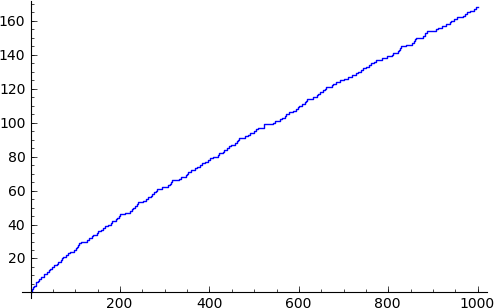
\includegraphics[scale=0.8]{images/prime-pi-1000}
\caption{Values of \texttt{prime\_pi(n)} for $n = 0, 1, 2, \dots, 1000$.}
\label{fig:number_theory:prime_pi_for_n_leq_1000}
\end{figure}


%%%%%%%%%%%%%%%%%%%%%%%%%%%%%%%%%%%%%%%%%%%%%%%%%%%%%%%%%%%%%%%%%%%%%%%%%%%

\section{Divisibility}

For any two integers $a$ and $n$, we say that $a$ \emph{divides} $n$
if $a$ is a factor of $n$. That is, if we can find an integer $b$ such
that $n = ab$, then $a$ is a factor of $n$. In that case, $b$ is also
a factor of $n$. The integer $2$ divides, or is a factor of, $4$
because $4 = 2 \times 2$. Similarly, both $2$ and $3$ are factors of,
or both divide, $6$ because $6 = 2 \times 3$.

Does every positive integer have a factor? Yes. In fact, if $n > 1$ is
an integer, then $n$ has a factor that is greater than $1$. We can
make a stronger claim: Every integer $n > 1$ has a prime factor. A
factorization, or prime factorization, of $n$ is product containing
all the primes that divide $n$. Examples of prime factorizations
include $4 = 2 \times 2$ and $6 = 2 \times 3$. However, $8 = 2 \times 4$
is not a prime factorization of $8$ because the product $2 \times 4$
has $4$, which is not prime.

To find all the positive divisors of an integer, use the command
\verb!divisors!.
%
\begin{lstlisting}
sage: divisors(4)
[1, 2, 4]
sage: divisors(6)
[1, 2, 3, 6]
sage: divisors(8)
[1, 2, 4, 8]
\end{lstlisting}
%
To write $n$ as a product of primes, use \verb!factor!.

\begin{lstlisting}
sage: factor(4)
2^2
sage: factor(6)
2 * 3
sage: factor(8)
2^3
\end{lstlisting}


%%%%%%%%%%%%%%%%%%%%%%%%%%%%%%%%%%%%%%%%%%%%%%%%%%%%%%%%%%%%%%%%%%%%%%%%%%%

\section{Greatest common divisors}

Let $a$ and $b$ be integers, not both zero. The \emph{greatest common}
divisor~(GCD) of $a$ and $b$ is the largest positive integer which is
a factor of both $a$ and $b$. We use $\gcd(a,b)$ to denote this
largest positive factor. If $n$ is any positive integer, then
$\gcd(n, 0) = n = \gcd(0, n)$. If $a$ and $b$ are both zero, then we
define their GCD to be $\gcd(0,0) = 0$. The GCD of any two distinct
primes is $1$, and the GCD of $18$ and $27$ is $9$.
%
\begin{lstlisting}
sage: gcd(0, 0)
0
sage: gcd(12, 0)
12
sage: gcd(13, 0)
13
sage: N = [1..20]; N
[1, 2, 3, 4, 5, 6, 7, 8, 9, 10, 11, 12, 13, 14, 15, 16, 17, 18, 19, 20]
sage: G = []
sage: for i in N:
...       G.append(gcd(i, 0))
sage: N
[1, 2, 3, 4, 5, 6, 7, 8, 9, 10, 11, 12, 13, 14, 15, 16, 17, 18, 19, 20]
sage: G
[1, 2, 3, 4, 5, 6, 7, 8, 9, 10, 11, 12, 13, 14, 15, 16, 17, 18, 19, 20]
\end{lstlisting}
%
In the above code listing, we used the command \verb![1..20]! to
obtain a list of all integers from $1$ to $20$, inclusive.

To find the GCD of $18$ and $27$, we could first use \verb!divisors!
to find the set of all positive divisors of each integer. We then
compare the set of divisors for $18$ with that for $27$, picking out
any integers that are common to both sets. From among all the divisors
that are common to both $18$ and $27$, we choose the largest such
divisor. The result is the GCD of $18$ and $27$.
%
\begin{lstlisting}
sage: D18 = Set(divisors(18)); D18
{1, 2, 3, 6, 9, 18}
sage: D27 = Set(divisors(27)); D27
{3, 1, 27, 9}
sage: D = D18.intersection(D27); D
{1, 3, 9}
sage: max(D)
9
\end{lstlisting}
%
The output of \verb!divisors! is a list. We used the command
\verb!Set! to convert the result of \verb!divisors! into a set. We
then used \verb!intersection! to produce the intersection of the two
sets \verb!D18! and \verb!D27!; this intersection is the set
\verb!D!. Finally, we used \verb!max! to compute the maximum element
in the set \verb!D!, i.e. $9$, the GCD we require.

Sage uses \verb!gcd(a, b)! to denote the GCD of $a$ and $b$. The GCD
of any two integers can be computed as follows:
%
\begin{lstlisting}
sage: gcd(3, 59)
1
sage: gcd(18, 27)
9
\end{lstlisting}

What about the case where any of $a$ and $b$ is negative? For example,
how do we compute the GCD of $-18$ and $27$, or $\gcd(-18, -27)$? If
$a$ is negative, for example, then we compute its
\emph{absolute value} and use that value to find the GCD of $a$ and
$b$. The absolute value of a number $x$ is written as $|x|$ and is
defined as
\[
|x|
=
\begin{cases}
x, & \text{if $x \geq 0$}, \\
-1 \times x, & \text{if $x < 0$}.
\end{cases}
\]
For example, the absolute value of $27$ is $|27| = 27$ because
$27 \geq 0$; the absolute value of $-18$ is
$|-18| = -1 \times (-18) = 18$ because $-18$ is negative. Then the GCD
of $-18$ and $27$ is
%
\begin{align*}
\gcd(-18, 27)
&=
\gcd(|-18|, 27) \\
&=
\gcd(18, 27) \\
&=
9.
\end{align*}

\begin{lstlisting}
sage: gcd(18, 27)
9
sage: gcd(-18, 27)
9
sage: gcd(-18, -27)
9
sage: # positive values of a, with b = 27
sage: N = [1..10]; N
[1, 2, 3, 4, 5, 6, 7, 8, 9, 10]
sage: G = []
sage: for i in N:
...       G.append(gcd(i, 27))
sage: G
[1, 1, 3, 1, 1, 3, 1, 1, 9, 1]
sage: # negative values of a, with b = 27
sage: N = [-1..-10, step=-1]; N
[-1, -2, -3, -4, -5, -6, -7, -8, -9, -10]
sage: G = []
sage: for i in N:
...       G.append(gcd(i, 27))
sage: G
[1, 1, 3, 1, 1, 3, 1, 1, 9, 1]
\end{lstlisting}

Figure~\ref{fig:number_theory:gcd_n_27} plots $\gcd(n, 27)$ for
integer values of $n$ from $1$ to $100$, inclusive. The horizontal
axis shows the values of $n$, while the vertical axis shows the values
of $\gcd(n, 27)$.

\begin{figure}[!htbp]
\centering
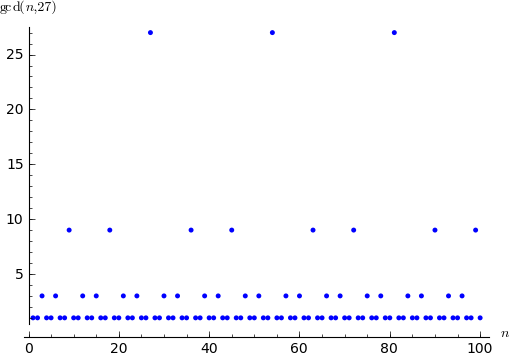
\includegraphics[scale=1.0]{images/gcd-100}
\caption{The GCD of $n$ and $27$ for $n = 1, 2, \dots, 100$.}
\label{fig:number_theory:gcd_n_27}
\end{figure}


%%%%%%%%%%%%%%%%%%%%%%%%%%%%%%%%%%%%%%%%%%%%%%%%%%%%%%%%%%%%%%%%%%%%%%%%%%%

\subsection{Relatively prime integers}

If $\gcd(a,b) = 1$, we say that $a$ is \emph{coprime}~(or relatively
prime) to $b$.  In particular, $\gcd(3, 59) = 1$ so 3 is coprime to 59
and vice versa.

Consider all the integers from 1 to 20, inclusive.  List all those
integers that are coprime to 20.  In other words, find those integers
$n$, where $1 \leq n \leq 20$, such that $\gcd(n,20) = 1$. The latter
task can be easily accomplished with a little bit of Sage programming:

\begin{lstlisting}
sage: for n in range(1, 21):
...       if gcd(n, 20) == 1:
...           print(n),
1 3 7 9 11 13 17 19
\end{lstlisting}

The above commands can be placed inside a function called
\verb!my_phi20! to save the hassle of retyping them everytime we want
to use those exact commands.

\begin{lstlisting}
sage: def my_phi20():
...       for n in range(1, 21):
...           if gcd(n, 20) == 1:
...               print(n),
sage: my_phi20()
1 3 7 9 11 13 17 19
\end{lstlisting}
%
From the output of \verb!my_phi20!, note that there are $8$ integers
between $1$ and $20$, inclusive, that are coprime to $20$. Without
explicitly generating the list
%
\begin{equation}
\label{eq:integers_coprime_to_20}
1 \quad 3 \quad 7 \quad 9 \quad 11 \quad 13 \quad 17 \quad 19
\end{equation}
%
how can we compute the number of integers between $1$ and $20$,
inclusive, that are coprime to 20? We could modify our function
\verb!my_phi20! so that it finds the number of positive integers that
are coprime to a given integer $n$.

\begin{lstlisting}
sage: def my_phi(n):
...       coprime = []
...       for i in range(1, n+1):
...           if gcd(i, n) == 1:
...               coprime.append(i)
...       return len(coprime)
sage: my_phi(20)
8
sage: my_phi(50)
20
sage: my_phi(100)
40
\end{lstlisting}

Alternatively, we could use the \emph{Euler phi function}
$\varphi(n)$, whose corresponding Sage built-in function is
\verb!euler_phi!.

\begin{lstlisting}
sage: euler_phi(20)
8
sage: euler_phi(50)
20
sage: euler_phi(100)
40
\end{lstlisting}
